\documentclass[conference]{IEEEtran}
\IEEEoverridecommandlockouts
% The preceding line is only needed to identify funding in the first footnote. If that is unneeded, please comment it out.
\usepackage{cite}
\usepackage{algorithmic}
\usepackage{graphicx}
\usepackage{textcomp}
\usepackage{amsmath}
\usepackage[sc]{mathpazo}
\usepackage{datetime}
\usepackage{graphicx, wrapfig, subcaption, setspace, booktabs}
\usepackage[T1]{fontenc}
\usepackage{fourier}
\usepackage{url, lipsum}
\usepackage{hyperref,bookmark}
\usepackage[T1]{fontenc}
\usepackage{amssymb}
\usepackage{makecell, multirow, tabularx}
\usepackage{listings}
\usepackage[ruled,linesnumbered,vlined]{algorithm2e}

\usepackage{float}
\usepackage{nomencl}
\usepackage{ifthen}

\renewcommand{\nomgroup}[1]{%
	\ifthenelse{\equal{#1}{P}}{\item[\textbf{Parameters}]}{%
		\ifthenelse{\equal{#1}{V}}{\item[\textbf{Variables \\}]}}
}
\makenomenclature
\def\BibTeX{{\rm B\kern-.05em{\sc i\kern-.025em b}\kern-.08em
    T\kern-.1667em\lower.7ex\hbox{E}\kern-.125emX}}
\begin{document}

\title{CO\textsubscript{2} Impact Electric Vehicle Charging on a Local Microgrid: a case study in Southern California }
%\Thanks{Identify Applicable Funding Agency Here. If None, Delete This.}
%}
%

%\author{\IEEEauthorblockN{1\textsuperscript{st}  Luis Fernando Enriquez-Contreras, Jacqueline Garrido,  Matthew Barth, Sadrul Ula, Arun Raju}
%	\IEEEauthorblockA{\textit{Department of Electrical  and Computer Engineering} \\
%		\textit{University of California, Riverside}\\
%		Riverside, United States of America \\
%		lenri001@ucr.edu, jgarr023@ucr.edu, barth@ece.ucr.edu, sula@cert.ucr.edu,  arun@engr.ucr.edu  }
%	\and
%	\IEEEauthorblockN{2\textsuperscript{nd} A S M Jahid Hasan}
%	\IEEEauthorblockA{\textit{Department of Electrical and Computer Engineering} \\
%		\textit{North South University}\\
%		Dhaka, Bangladesh\\
%		jahid.hasan12@northsouth.edu }
%	\and
%	\IEEEauthorblockN{3\textsuperscript{rd} Jubair Yusuf}
%	\IEEEauthorblockA{\textit{Electric Power Systems Research} \\
%		\textit{Sandia National Laboratories}\\
%		Albuquerque,  United States of America\\
%		jyusuf@sandia.gov}
%
%
%}

\author{
	\IEEEauthorblockN{1\textsuperscript{st} Luis Fernando Enriquez-Contreras\IEEEauthorrefmark{1}\IEEEauthorrefmark{2}, Jacqueline Garrido\IEEEauthorrefmark{1}\IEEEauthorrefmark{2}, Matthew Barth\IEEEauthorrefmark{1}\IEEEauthorrefmark{2}, Sadrul Ula\IEEEauthorrefmark{2}, Arun Raju\IEEEauthorrefmark{2}}
	\IEEEauthorblockA{\IEEEauthorrefmark{1}\textit{Department of Electrical  and Computer Engineering} \\
		\textit{University of California, Riverside}\\
				Riverside, United States of America \\
				lenri001@ucr.edu, jgarr023@ucr.edu, barth@ece.ucr.edu}
	\IEEEauthorblockA{\IEEEauthorrefmark{2}\textit{College of Engineering, Center for Environmental Research \& Technology} \\
		\textit{University of California, Riverside}\\
				Riverside, United States of America \\
				lenri001@ucr.edu, jgarr023@ucr.edu, barth@ece.ucr.edu, sula@cert.ucr.edu,  arun@engr.ucr.edu}
		\and
	\IEEEauthorblockN{2\textsuperscript{nd} A S M Jahid Hasan}
	\IEEEauthorblockA{\textit{Department of Electrical and Computer Engineering} \\
			\textit{North South University}\\
			Dhaka, Bangladesh\\
			jahid.hasan12@northsouth.edu }
		\and
	\IEEEauthorblockN{3\textsuperscript{rd} Jubair Yusuf}
	\IEEEauthorblockA{\textit{Department of Electrical  and Computer Engineering} \\
			\textit{University of California, Riverside}\\
			Riverside,  United States of America\\
			jyusu001@ucr.edu}
}
\maketitle

\begin{abstract}

		As renewable energy penetration in electric grids increases with time, it becomes more important for electric utilities to update their electric rates  such that they minimize CO\textsubscript{2} emissions. In this paper, we evaluate a case study at the University of California, Riverside (UCR) to simulate different Time of Use (TOU) rate optimizations that minimizes electric costs while analyzing CO\textsubscript{2} output, by using the openmodelica model, we based on different electric utility rates in Southern California.  The different amounts of power and energy consumed by each rate is compared with CAISO CO\textsubscript{2} emissions data in order to review the different emission levels from the different utility electric rates on a 15 minute basis.  Electric costs are also compared in order to see the different savings the consumer will have with the different rates. It was found that Southern California Edison (SCE) TOU rate had the most savings for the consumer and that Riverside (RPU) TOU flat rate had the lowest CO\textsubscript{2} emissions.

\end{abstract}

\begin{IEEEkeywords}
micorgrids, demand response, TOU, CO\textsubscript{2} emissions, modelica
\end{IEEEkeywords}

%Parameters

%\nomenclature[P0]{$t$}{Timestep in seconds}
%
%\nomenclature[P1]{$\Delta t$}{Duration of each timestep}
%
%\nomenclature[P2]{$T^{\prime}$}{Total number of timesteps}
%
%\nomenclature[P3]{$E_{\text {init }}^{B}$}{Initial stored energy of the BESS}
%
%\nomenclature[P4]{$P_{t}^{S}$}{Solar generation $\mathrm{t}$}
%
%\nomenclature[P5]{$P_{t}^{L}$}{Load at $\mathrm{t}$}
%
%\nomenclature[P6]{$\alpha_{t}$}{Energy charge at $\mathrm{t}$}
%
%\nomenclature[P7]{$\beta$}{Monthly peak demand charge}
%
%\nomenclature[P8]{$\beta_{t}^{\text {On }} / \beta_{t}^{\text {Mid }} / \beta_{t}^{\text {Off }}$}{$\mathrm{On} / \mathrm{Mid} / $Off-Peak demand charges at $\mathrm{t}$}
%
%\nomenclature[P8]{$\eta^{+} / \eta^{-}$}{Charging/discharging efficiency of BESS}
%
%%Variables
%\nomenclature[Vx]{}{}
%\nomenclature[V0]{$E_{t}^{B}$}{Energy stored at $\mathrm{t}$ in BESS}
%
%\nomenclature[V1]{$P_{t}^{B}$}{BESS power at $\mathrm{t}$}
%
%\nomenclature[V2]{$P_{t}^{B+} / P_{t}^{B-}$}{BESS charging/discharging power at $\mathrm{t}$}
%
%\nomenclature[V3]{$P_{t}^{G}$}{Power drawn from the grid at $\mathrm{t}$}
%
%\nomenclature[V4]{$P_{t}^{S B}$}{Solar power fed to BESS at $\mathrm{t}$}
%
%\nomenclature[V5]{$P_{t}^{S L}$}{Solar power fed to load at $\mathrm{t}$}
%
%\nomenclature[V6]{$P_{t}^{B L}$}{BESS power fed to load at $\mathrm{t}$}
%
%\printnomenclature
\section{Introduction}
    \subsection{Background}
%     			California is going through a major transition in energy production, which involves a higher share of renewable energy in the electricity mix. This is to meet California's climate goals of a 48\% reduction in greenhouse gas by 2030 \cite{California_2022}. However, achieving that goal will involve utility companies, government agencies, and consumers to all play a role. Many industrial and commercial sites are not only installing solar power, but introducing battery energy storage systems (BESS) as well. Since January 2023, California law requires new commercial buildings to have solar and battery storage systems installed  \cite{PowerFlex_2023}. This has major potential in addressing current issues associated with solar power as a large percentage of the energy mix. The infamous duck curve has only been getting steeper in recent years to the point it is being called a canyon curve \cite{canyon_curve}, leading to a huge stress onto the grid and concerns about reliability \cite{eia} \cite{caiso_duck}. Equally as important, while California has a relatively clean grid during solar peak production hours, the electrical demand does not align with these low CO\textsubscript{2} emissions times and relies on the grid during when CO\textsubscript{2} emissions are higher. BESS have been proposed as one of the solutions to mitigate the duck curve problems. This paper reviews rates (flat, TOU) of various utility companies coupled with a typical microgrid at UC Riverside to compare how customers using a BESS for both economic benefit, and as a means of reducing CO\textsubscript{2} emissions. \\
  	\subsection{Literature Review}
%			Previous literature has explored various topics concerning TOU impacts on  CO\textsubscript{2} emissions. In \cite{schedulingcontroller}, a lightning search algorithm (LSA) is used to optimize a microgrid controller based on CO\textsubscript{2} emissions, energy use, and demand costs. Their model predicts a reduction of 78 to 220 tons of CO\textsubscript{2} from the atmosphere, does not optimize using TOU rates, and calculates emissions using a flat demand. In \cite{economicandenvironmentalpolicy}, the authors investigate the deployment cost of multiple scenarios in a multi-carrier microgrid (MCMG) model that considers demand shifting, monthly peak, and CO\textsubscript{2} emissions. They advocate for better environmental policies in the utility sector since the MCMG scenario optimized solely for CO\textsubscript{2} emissions was 39\% less cost-effective than the scenario optimized for cost.  In  \cite{stochasticoptimalscheduling}, simulations are run on a system consisting of three microgrids while considering and neglecting emission charges. CO\textsubscript{2} Emissions were halved when considering CO\textsubscript{2} emissions charges. However, the lower emission operation has a higher upfront cost and is less economically attractive for customers. In \cite{emsformg} five scenarios with cost and emission reduction in mind are done in an isolated microgrid. The authors conclude that running the pareto control strategy is the best compromise between cost and CO\textsubscript{2} emissions output. The different case scenarios were different balances between cost and CO\textsubscript{2} emissions, but only used one electric rate. In \cite{abcdr}, the authors assess different demand side management strategies utilizing the Artificial Bee Colony algorithm under different tariff structures. TOU, critical peak pricing (CPP), real-time electricity pricing (RTEP), and day-ahead pricing (DAP) seasonal pricing structures were assessed for CO\textsubscript{2} emissions output using demand side management and no BESS. \cite{optimalmmgemissions} compares microgrids considering demand response and/or electricity sharing and compares those scenarios by the amount of costs and carbon CO\textsubscript{2} emissions. This paper incorporates the different aspects of these papers, as shown in Figure \ref{tab:litreview}.
%			\\
%			\begin{table}[H]
%			\caption{Contributions of Various Papers in  the CO\textsubscript{2} Emissions of Electric Grids }
%			\tiny
%				\begin{tabularx}{\linewidth}{X | l | l | l | l | l} 
		\hline
		Paper & Flat Rate  &  Emissions Output &  TOU & BESS & Utility Pricing Structure  \\ 
		\hline\hline
		\cite{schedulingcontroller} & X & \checkmark  & \checkmark &  \checkmark  &  X\\ 
		\hline
		\cite{economicandenvironmentalpolicy} & \checkmark & \checkmark & \checkmark & \checkmark & X \\
		\hline
		\cite{stochasticoptimalscheduling} & \checkmark & \checkmark  &  \checkmark & \checkmark & X \\
		\hline
		\cite{emsformg} & \checkmark& \checkmark&  \checkmark  & \checkmark & X \\
		\hline
		\cite{abcdr} & \checkmark &  \checkmark & \checkmark  & X  & \checkmark\\ 
		\hline
		\cite{optimalmmgemissions} & \checkmark& \checkmark&  \checkmark  & X & X \\
		\hline
		\cite{garrido2021dynamic} & \checkmark & \checkmark & \checkmark & X & \checkmark \\ 
		\hline
		\cite{hasan2023universal} & \checkmark & X & \checkmark & \checkmark & \checkmark \\
		\hline
		\cite{enriquez2022microgrid} & \checkmark & X & \checkmark & \checkmark & \checkmark \\
		\hline
		This Paper & \checkmark & \checkmark  & \checkmark &  \checkmark & \checkmark \\ 
		\hline
	\end{tabularx}
%			\normalsize
%			\label{tab:litreview}
%			\end{table}
			This paper's main contribution is to analyze the impacts different pricing structures have on the behavior of microgrids and the associated CO\textsubscript{2} emissions. One goal every TOU pricing schedule should have is for the economic incentives to align with CO\textsubscript{2} emission reductions. This paper evaluates flat rate and TOU pricing from different electric utilities in California. This paper also uses a higher time resolution than most to date and explains in further detail of a realistic simulation of a microgrid using system dynamics software.  
    \subsection{Pricing (Flat vs TOU)}
%      		One of the main contributions of this paper is to see how a flat rate versus TOU pricing affects the CO\textsubscript{2} emissions associated with adapting different rate schedules. A flat rate demand charge means the customer is charged for the maximum power consumed within a 15-minute rolling average, regardless of when this maximum occurs. A TOU rate means the customer has a charge for the maximum amount of power used if any 15-minute rolling average within each of the predefined blocks, usually off-peak, mid-peak, on-peak, and any depending on the season super off-peak. In our case study, the microgrid electric rate is the RPU flat demand charge; however,  we simulate other pricing scenarios, including the RPU TOU rate, and investor-owned utilities (IOU) TOU rates. TOU rates can be seasonal, meaning the rate peak times change depending on the season. All rates in this case study utilize the summer seasonal rate since it is usually when the grid is the most strained and electric utilities are the least flexible to changing the times, and when the month of x is analyzed. The customer is usually charged for both demand and energy charges in commercial rates. Energy charges are similar to demand charges since they both use the same TOU time period but differ in that energy charges are the sum of energy for that time period compared to the maximum demand during the TOU period for demand charges. The SCE and Los Angeles Department of Water of Power (LADWP) rate schedules are analyzed in this paper as they are the other two major electric utilities in Southern California. The different rates used in this study are shown in Table \ref{tab:electricpricing}.
%       		\begin{table}[H]
%       			\caption{TOU Schedule Rates in Southern California }
%       			\footnotesize
%       			\begin{tabularx}{\linewidth}{X|X|l | l | l }
\toprule
          & &  RPU &   LADWP   &  SCE  \\
\midrule
	\parbox[t]{5mm}{\multirow{3}{*}{\rotatebox[origin=X]{90}{\makecell{Demand \\ Charges \\ (\$)} }}} &
        Off-Peak  &  1.85   &   0  &  0     \\
        & Mid-Peak   &  3.69  &   3.75  &   0     \\
        & On-Peak    &  7.38 &   10 &  18.11    \\
     \parbox[t]{5mm}{\multirow{3}{*}{\rotatebox[origin=X]{90}{ \makecell{Energy \\ Charges \\ (\$)} }}} &
        Off-Peak   &  0.0808 &   0.03522 &  0.03712    \\
        & Mid-Peak   &  0.0946 & 0.05595 &  0.06412    \\
        & On-Peak   &  0.1154  &  0.06322 &   0.07275     \\
       \parbox[t]{5mm}{\multirow{3}{*}{\rotatebox[origin=X]{90}{\makecell{TOU Hours} }}} &
        Off-Peak  &  0 - 8, 23 - 0  & 0 - 10, 20 - 0  &   0 - 16, 21 - 0   \\
        & Mid-Peak  & 8 - 12, 18 - 23  &  10 - 13, 17 - 20  &   N/A     \\
        & On-Peak  & 12 - 18 & 13 - 17  &  16 - 21  \\  
\bottomrule
\end{tabularx}

%       			\normalsize
%       			\label{tab:electricpricing}
%       		\end{table}

    \subsection{Peak Shaving Strategy}
       		Peak shaving is a standard method for reducing high-demand charges. Since demand charges are based on only the maximum value over the entire month, in this simple algorithm, we assume the consumer wants to minimize the demand charges as much as possible. The algorithm is based solely on cost savings for a typical microgrid. During flat-rate peak shaving, the algorithm looks at the amount of power being imported, if there is enough energy, and if the batteries can mitigate a fraction of that or the total amount. With TOU, peak shaving is prioritized more during on-peak times, and shifts demand to mid-peak and off-peak hours. 
    \subsection{CO\textsubscript{2} Emissions}
        	Our microgrid's solar production greatly overlaps with the local solar energy production within the larger grid. This leads to the problem within our microgrid that while it is zero CO\textsubscript{2} emissions during solar peak hours we still rely on the 30 main electrical grid during off peak hours, which is when there are higher CO\textsubscript{2} emissions. However, with a BESS, we can utilize renewable energy during peak times and at night. In this scenario, the control algorithm is economic-based since we want to see how  the TOU rates align with actual CO\textsubscript{2} emissions output. The simulation uses emission output calculations from CAISO for each time interval, as a sum of all the powerplant CO\textsubscript{2} emissions (imports, natural gas, biogas, biomass, geothermal, coal) \textsubscript{m}TON\textsubscript{CO\textsubscript{2}} / hour. The CO\textsubscript{2} emissions output is divided by the amount of power produced (solar, wind, geothermal, biomass, biogas, small hydro, grid batteries, large hydro, imports, nuclear, coal ) in MW, which gives us an emissions rate of (TON\textsubscript{CO\textsubscript{2}} / hour) / W. This is multiplied with our 15-minute data kW, and a multiplier of  $1/ 4000$ to convert kW into W and to address for the 4 15 minute periods in an hour.   This gives us an estimate of the amount of CO\textsubscript{2} emissions in \textsubscript{m}TON\textsubscript{CO\textsubscript{2}} for every 15 minutes that is summed together to give us the total for the entire period.  This method is similar to the one used in \cite{garrido2021dynamic}.  When the grid does not pull power from the grid or is sending power, the CO\textsubscript{2} emissions are assumed to be zero, since we are using our solar energy.
\section{Simulation in OpenModelica}
    	Openmodelica is an open-source implementation of the Modelica programming language \cite{OpenModelica}. Modelica is a programming language that is designed for dynamic systems simulation \cite{ModelicaLanguage}. OMEdit is the GUI interface for open Modelica, allowing the user to draw a system for simulation \cite{OMEdit}. The microgrid scenarios are simulated in open Modelica using the Modelica buildings library.  Lawrence Berkeley National Laboratory created the Modelica buildings library for building and district energy and control systems \cite{ModelicaBuildingsLibrary}. However, its capability for energy storage systems, bi-directional inverter, solar, and HVAC modeling make it ideal for a microgrid simulation setup. This allows us to create scenarios that do not currently exist in our microgrid, like running a month with solar with the same load, or running the BESS control algorithm for different electric rates.  The power circuits are three-phase balanced circuits. The simulation of our case study microgrid is the grid-connected to the building netload. The model's net load is broken down into solar power, HVAC loads, regular building loads, electric vehicle chargers, and the BESS as shown in Figure \ref{fig:powersystemsetupfull} . 
	\begin{figure}[H]
		\centering
		\includegraphics[width=1\linewidth]{Fig/power_system_setup_modelica}
		\caption{Microgrid Layout}
		\label{fig:powersystemsetupfull}
	\end{figure}
	\subsection{Validation}
		To ensure that our model accurately portrays our real world system, a year of real world data was used to validate the $P_G $ output . $P_G$ is defined as the power the microgrid sends or consume from the grid.  The actual data was compared to the simulated  with a correlation coefficient of  $\approx$ 0.965087 as shown in Figure \ref{fig:ucr15minutedatamar012022tomar012023}. 
		\begin{figure}[H]
			\centering
			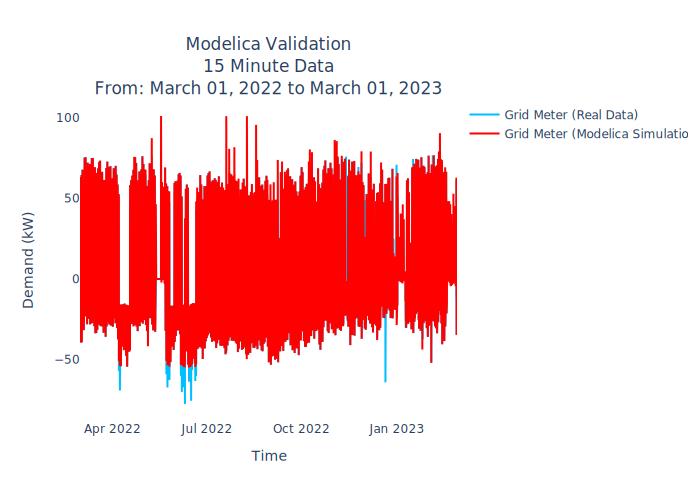
\includegraphics[width=1\linewidth]{Fig/ucr_15_Minute_Data_Mar_01_2022_to_Mar_01_2023}
			\caption{Whole Year Validation}
			\label{fig:ucr15minutedatamar012022tomar012023}
		\end{figure}
		
    \subsection{Solar Generation and Building Loads}
    	The solar power in our model is based on the historical solar data from our PV array. The HVAC loads and the regular building loads are represented separately in this model but utilize the same method; they both use historical real world power data to represent a their load in the system. 
    \subsection{EV Charger Loads }
   		Our model also considers transportation loads in the form of EV chargers. The EV chargers are represented as two models: Level 2 EV chargers, and Level 3 EV chargers. While other loads follow a typical daily and yearly pattern, EV loads are different since they switch on and off. Our case study microgrid has four Level 2 chargers, so it can have four ``steps'' of 7.2 kW each, while there is only one ``step'' of 50 kW with the Level 3 chargers. To generate EV loads, we use a Poisson random generator to generate the number of charge sessions in a day, the arrival times, and charging durations based on real world data. 
		\begin{figure}[H]
			\centering
			\includegraphics[width=1\linewidth]{Fig/l2_avg_day_rand_poisson_1_hour_pdf}
			\caption{Probability Density Function of the Level 2 EV Charger Validation}
			\label{fig:l2avgdayrandpoisson1hourpdf}
		\end{figure}

%   		However, the number of sessions and duration is reduced to X and Y for the Level 3 charger.  
%		\begin{figure}[H]
%			\centering
%			\includegraphics[width=1\linewidth]{Fig/l2_avg_day_rand_poisson_1_hour}
%			\caption{Number of Real and Simulated Sessions}
%			\label{fig:l2avgdayrandpoisson1hour}
%		\end{figure}
		
		Historical data was collected from the Level-2 charger to determine the parameters for the Poisson random generator, following a typical daily charge pdf shown in Figure \ref{fig:l2avgdayrandpoisson1hourpdf}, and the power output of the Level 2 chargers in Figure \ref{fig:l2gpadpoissonjune}. 
		
			\begin{figure}[H]
				\centering
				\includegraphics[width=1\linewidth]{Fig/l2_g_pad_poisson_June}
				\caption{Level 2 Chargers Simulated Power Output}
				\label{fig:l2gpadpoissonjune}
			\end{figure}
%		\begin{figure}[H]
%			\centering
%			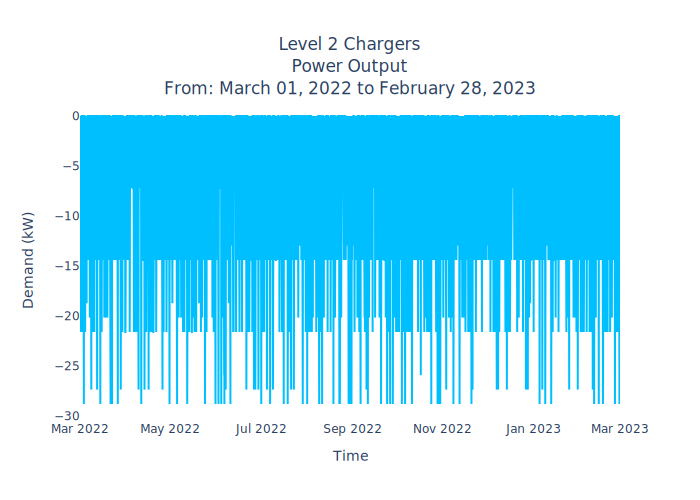
\includegraphics[width=1\linewidth]{Fig/ev_l2_po}
%			\caption{Level 2 Power Output}
%			\label{fig:evl2po}
%		\end{figure}
    
    \subsection{BESS and Peak Shaving}
    	The BESS is modeled as a battery connected to a bidirectional inverter. The BESS output is controlled by generated data from the control algorithm. The BESS output is computed in real-time by using a peak shaving algorithm utilizing  BESS SOC and the grid meter output. The algorithm charges the battery when excess solar power is exported to the grid, and the battery needs to be charged. Python code reads the net load from the grid  model and determines the amount of CO\textsubscript{2} being produced during that interval.  Algorithm \ref{alg:peakshavingflatrate} shows the peak shaving algorithm sufficient for flat rate demand response. 
%    	However,  for a TOU pricing structure, both energy and demand charges are assumed to be TOU rates with no additional flat rate demands. The TOU peak shaving algorithm is presented in Equation 1 with a simple objective to minimize the amount of power the microgrid pulls from the grid while accounting for energy and demand charges. The minimization objective is accomplished by optimizing for the summation of  TOU energy ($\Delta t \boldsymbol{\alpha}^{\boldsymbol{T}} \boldsymbol{P}^G$) and the maximums TOU demands ($\max \left(\boldsymbol{\beta}^{\text {On }} \boldsymbol{P}^G\right)+\max \left(\boldsymbol{\beta}^{\text {Mid }} \boldsymbol{P}^G\right)+\max \left(\boldsymbol{\beta}^{\text {Off }} \boldsymbol{P}^G\right)$). This algorithm is further described and validated in \cite{hasan2023universal},  \cite{hasan2021comprehensive} . \\
%%		\begin{figure}
%%			\centering
%%			\includegraphics[width=0.7\linewidth]{Fig/peak_shaving_flat_rate}
%%			\caption{Flat Rate Peak Shaving Algorithm Flowchart}
%%			\label{fig:peakshavingflatrate}
%%		\end{figure}
%			\normalsize
%			\footnotesize
%		\begin{equation} 
%			\min f\left(\boldsymbol{P}^G\right)=\Delta t \boldsymbol{\alpha}^{\boldsymbol{T}} \boldsymbol{P}^G+\max \left(\boldsymbol{\beta}^{\text {On }} \boldsymbol{P}^G\right)+\max \left(\boldsymbol{\beta}^{\text {Mid }} \boldsymbol{P}^G\right)+\max \left(\boldsymbol{\beta}^{\text {Off }} \boldsymbol{P}^G\right)
%		\end{equation}
%		\normalsize
%		subject to
%		$$
%		\begin{aligned}
%			& E_{t+1}^B=E_t^B+P_t^B \cdot \Delta t, \forall t \in \boldsymbol{T}^{\mathbf{t o t}} \\
%			& E^{B m i n} \leq E_t^B \leq E^{B m a x}, \forall t \in \boldsymbol{T}^{\mathbf{t o t}} \\
%			& P_t^B=P_t^{B+}-P_t^{B-}, \forall t \in \boldsymbol{T}^{\text {tot }} \\
%			& 0 \leq P_t^{B+} \leq \delta_t P^{B+\max }, \forall t \in \boldsymbol{T}^{\mathbf{t o t}} \\
%			& 0 \leq P_t^{B-} \leq\left(1-\delta_t\right) P^{B-\max }, \forall t \in \boldsymbol{T}^{\mathbf{t o t}} \\
%			& 0 \leq \delta_t \leq 1, \forall t \in \boldsymbol{T}^{\mathbf{t o t}} \\
%			& P_t^{B+}=\eta^{+} P_t^{S B}, \forall t \in \boldsymbol{T}^{\mathbf{t o t}} \\
%			& P_t^S=P_t^{S B}+P_t^{S L}, \forall t \in \boldsymbol{T}^{t o t} \\
%			& P_t^L=P_t^{S L}+P_t^{B L}+P_t^G, \forall t \in \boldsymbol{T}^{\text {tot }} \\
%			& P_t^{B L}=\eta^{-} P_t^{B-}, \forall t \in \boldsymbol{T}^{t o t} \\
%			& P_t^{S L} \geq 0, \forall t \in \boldsymbol{T}^{t o t}
%		\end{aligned}
%		$$

		\begin{algorithm}
			net\_load, SOC $\gets$ Modelica Data Output
			\uIf{if condition}{net\_load  <=   -15 kW and SOC > 20 \%  and net\_load  >=  -100 kW
				BESS\_inverter = -net\_load  - 15 kW
			}
			\uElseIf{net\_load  <= -100 kW and SOC > 20 \%}{
					BESS\_inverter = -100 kW
			}
			\uElseIf{net\_load  >=  0 kW and SOC < 90 \%  and net\_load  <=  100 kW}{ 
				 BESS\_inverter = -net\_load
			}
			\uElseIf{net\_load  >=  0 kW and SOC < 90 \%  }{
				 BESS\_inverter = 100 kW
			}
			\Else{
				BESS\_inverter = 0
			}
			\caption{Peak Shaving}
			\label{alg:peakshavingflatrate}
		\end{algorithm}
%		\begin{algorithm}
%			\caption{Flat Rate Peak-Shaving}}\label{alg:peak_shaving}
%			df $\gets$ dataset \\
%			output $\gets$ [] \\
%			count $\gets$ 0 \\
%			delay $\gets$ 15 minutes \\
%			new\_interval $\gets$ current\_time \\
%			\uIf {data\_length $>$ count}{
%			}
%			\uElseIf{}{
%			}	
%			\uElseIf{}{
%			}	
%			\uElseIf{}{
%			}
%			\Else{
%			}	
%		\end{algorithm}
	
\section{Results}
%    \subsection{Scenarios}

%    	\subsubsection{Scenario 1}   		
%    					\begin{figure*}
%    			\centering
%    			\begin{subfigure}[b]{0.475\textwidth}
%    				\centering
%    				\includegraphics[width=\textwidth]{Fig/ucr_theortical_actual_net_load_11_20.pdf}
%    				\caption[Network2]%
%    				{{\small UCR Microgrid Building Theoretical and Actual Load Data }}    
%    				\label{ucr_act}
%    			\end{subfigure}
%    			\hfill
%    			\begin{subfigure}[b]{0.475\textwidth}  
%    				\centering 
%    				\includegraphics[width=\textwidth]{Fig/ucr_theortical_actual_net_load_resample_11_20.pdf}
%    				\caption[]%
%    				{{\small UCR Microgrid Building Theoretical and Actual Load 15 Minute Average Resample}}    
%    				\label{ucr_act_rs}
%    			\end{subfigure}
%    			\vskip\baselineskip
%    			
%    			\caption[ The average and standard deviation of critical parameters ]
%    			{\small UCR Microgrid Building Theoretical and Actual Load} 
%    			\label{fig:ucr_act}
%    		\end{figure*}

%		\begin{figure*}
%				\begin{subfigure}[b]{0.475\textwidth}
%					\centering
%					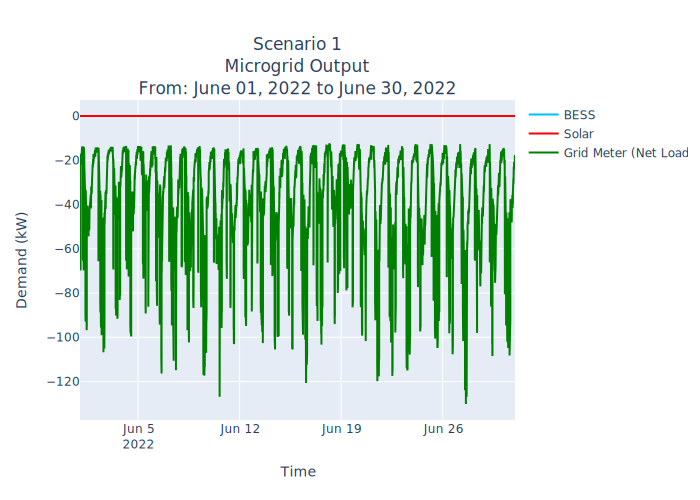
\includegraphics[width=1\linewidth]{Fig/3_Scenario_1_Mg_Output_Jun_01_2022_to_Jun_30_2022}
%					\caption{Scenario 1}
%					\label{fig:3scenario1mgoutputjun012022tojun302022}
%				\end{subfigure}
%				\hfill
%				\begin{subfigure}[b]{0.475\textwidth}
%					\centering
%					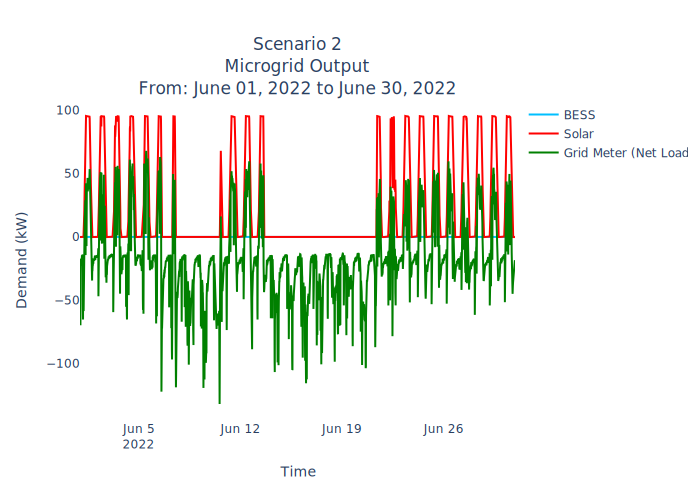
\includegraphics[width=1\linewidth]{Fig/3_Scenario_2_Mg_Output_Jun_01_2022_to_Jun_30_2022}
%					\caption{Scenario 2}
%					\label{fig:3scenario2mgoutputjun012022tojun302022}
%				\end{subfigure}			
%				
%				\begin{subfigure}[b]{0.475\textwidth}
%					\centering
%					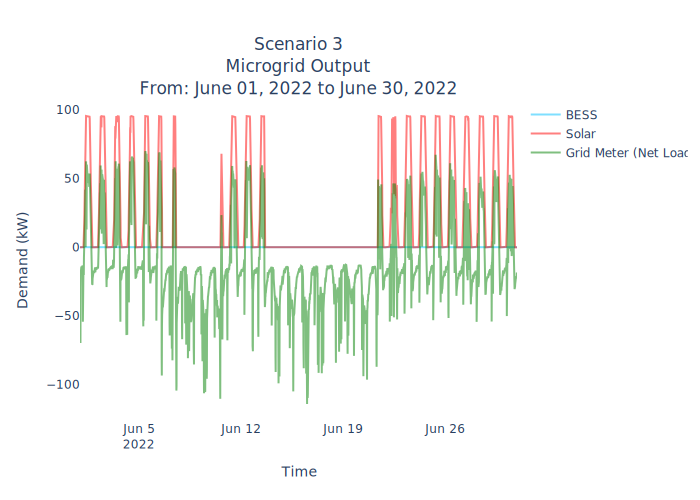
\includegraphics[width=1\linewidth]{Fig/3_Scenario_3_Mg_Output_Jun_01_2022_to_Jun_30_2022}
%					\caption{Scenario 3}
%					\label{fig:3scenario3mgoutputjun012022tojun302022}
%				\end{subfigure}
%				\hfill
%				\begin{subfigure}[b]{0.475\textwidth}
%					\centering
%					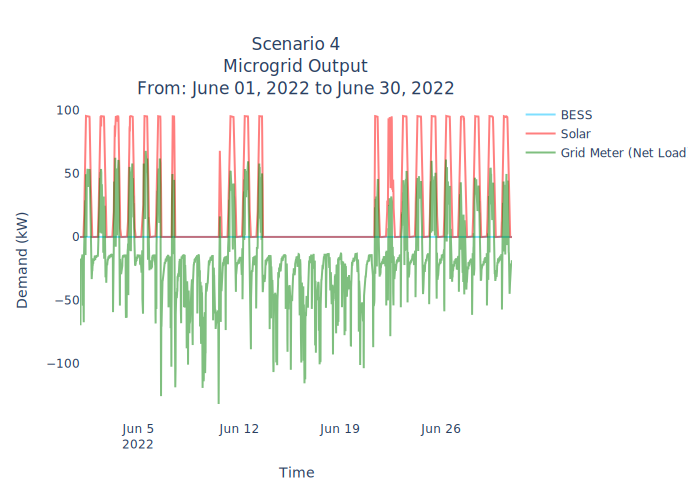
\includegraphics[width=1\linewidth]{Fig/3_Scenario_4_Mg_Output_Jun_01_2022_to_Jun_30_2022}
%					\caption{Scenario 4}
%					\label{fig:3scenario4mgoutputjun012022tojun302022}
%				\end{subfigure}				
%				
%				\begin{subfigure}[b]{0.475\textwidth}
%					\centering
%					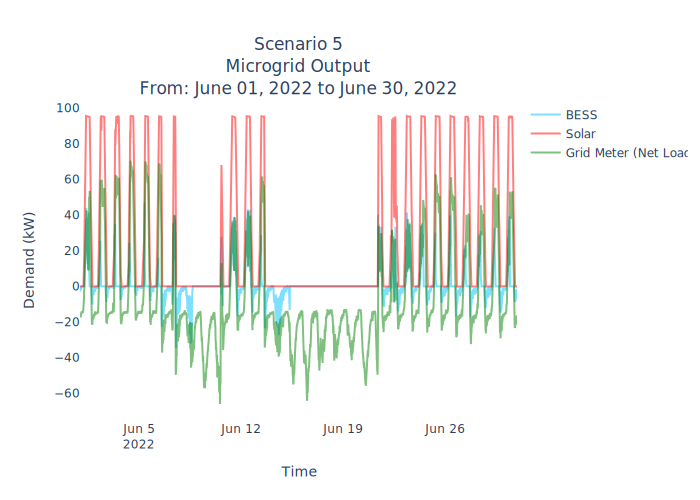
\includegraphics[width=1\linewidth]{Fig/3_Scenario_5_Mg_Output_Jun_01_2022_to_Jun_30_2022}
%					\caption{Scenario 5}
%					\label{fig:3scenario5mgoutputjun012022tojun302022}
%				\end{subfigure}				
%				\hfill
%				\begin{subfigure}[b]{0.475\textwidth}
%					\centering
%					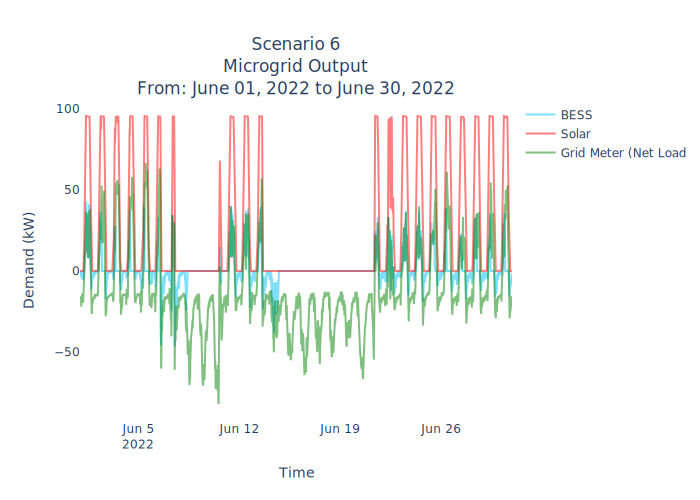
\includegraphics[width=1\linewidth]{Fig/3_Scenario_6_Mg_Output_Jun_01_2022_to_Jun_30_2022}
%					\caption{Scenario 6}
%					\label{fig:3scenario6mgoutputjun012022tojun302022}
%				\end{subfigure}
%		\end{figure*}
%				
%				\begin{figure}[H]
%					\centering
%					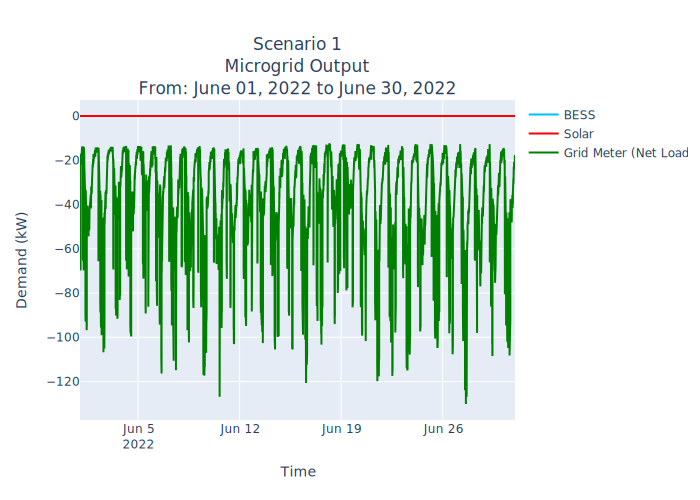
\includegraphics[width=1\linewidth]{Fig/3_Scenario_1_Mg_Output_Jun_01_2022_to_Jun_30_2022}
%					\caption{Scenario 1}
%					\label{fig:3scenario1mgoutputjun012022tojun302022}
%				\end{figure}
%				
%				\begin{figure}[H]
%					\centering
%					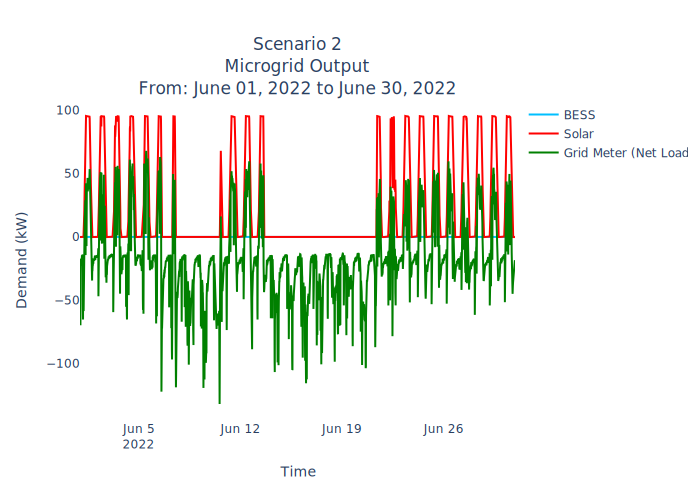
\includegraphics[width=1\linewidth]{Fig/3_Scenario_2_Mg_Output_Jun_01_2022_to_Jun_30_2022}
%					\caption{Scenario 2}
%					\label{fig:3scenario2mgoutputjun012022tojun302022}
%				\end{figure}			
%				
%				\begin{figure}[H]
%					\centering
%					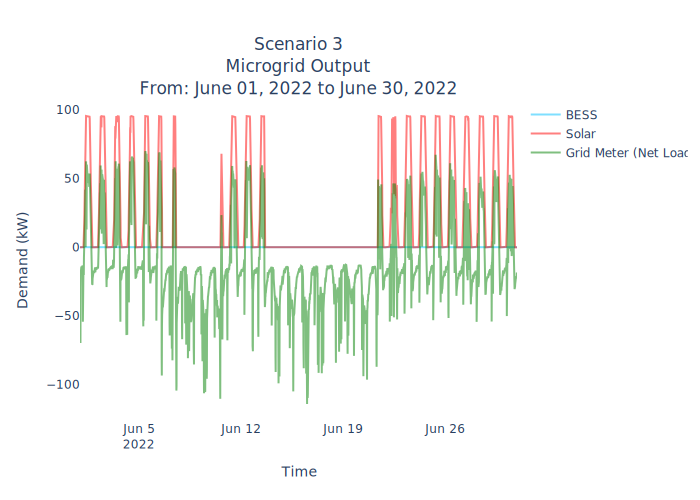
\includegraphics[width=1\linewidth]{Fig/3_Scenario_3_Mg_Output_Jun_01_2022_to_Jun_30_2022}
%					\caption{Scenario 3}
%					\label{fig:3scenario3mgoutputjun012022tojun302022}
%				\end{figure}
%				
%				\begin{figure}[H]
%					\centering
%					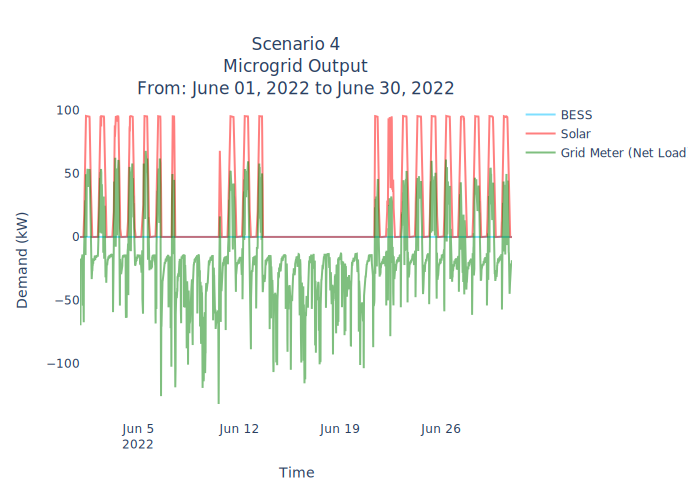
\includegraphics[width=1\linewidth]{Fig/3_Scenario_4_Mg_Output_Jun_01_2022_to_Jun_30_2022}
%					\caption{Scenario 4}
%					\label{fig:3scenario4mgoutputjun012022tojun302022}
%				\end{figure}				
%				
%				\begin{figure}[H]
%					\centering
%					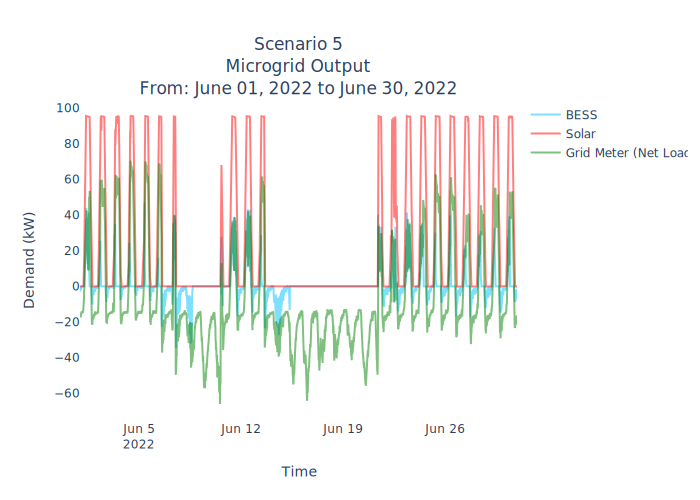
\includegraphics[width=1\linewidth]{Fig/3_Scenario_5_Mg_Output_Jun_01_2022_to_Jun_30_2022}
%					\caption{Scenario 5}
%					\label{fig:3scenario5mgoutputjun012022tojun302022}
%				\end{figure}				
%				
%				\begin{figure}[H]
%					\centering
%					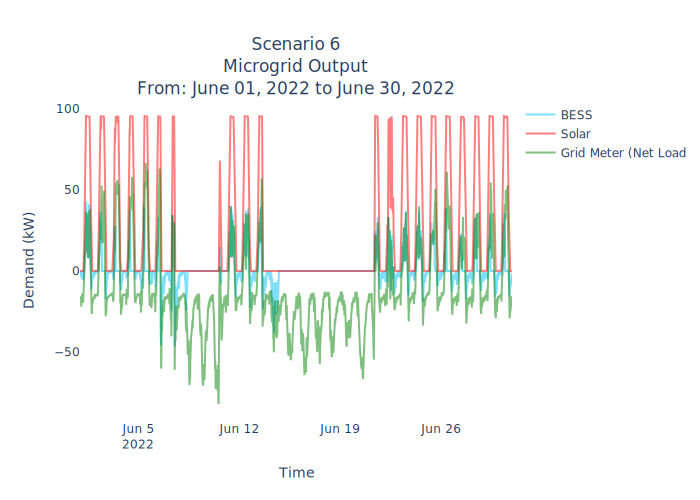
\includegraphics[width=1\linewidth]{Fig/3_Scenario_6_Mg_Output_Jun_01_2022_to_Jun_30_2022}
%					\caption{Scenario 6}
%					\label{fig:3scenario6mgoutputjun012022tojun302022}
%				\end{figure}
				
				
%			\begin{figure}[H]
%				\centering
%				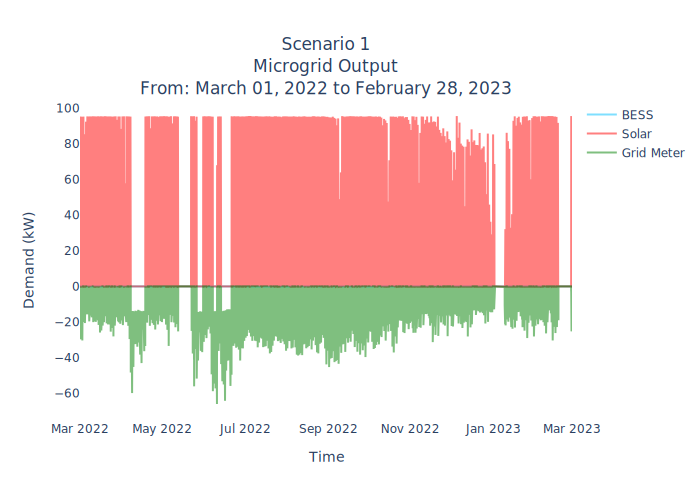
\includegraphics[width=1\linewidth]{Fig/0_Mg_Output_Mar_01_2022_to_Feb_28_2023}
%				\caption{}
%				\label{fig:0mgoutputmar012022tofeb282023}
%			\end{figure}
%    	\subsubsection{Scenario 2}
%			\begin{figure}[H]
%				\centering
%				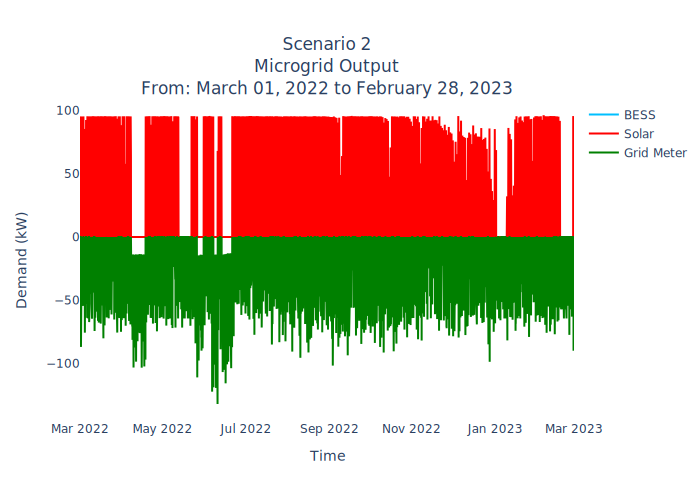
\includegraphics[width=1\linewidth]{Fig/1_Mg_Output_Mar_01_2022_to_Feb_28_2023}
%				\caption{}
%				\label{fig:1mgoutputmar012022tofeb282023}
%			\end{figure}
%    	\subsubsection{Scenario 3}
%			\begin{figure}[H]
%				\centering
%				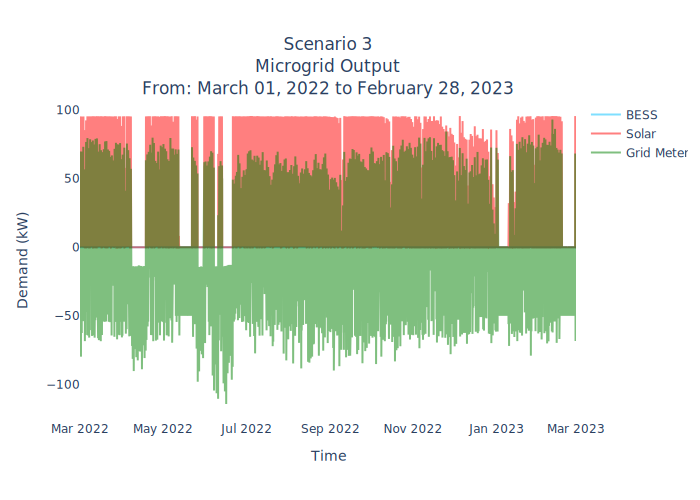
\includegraphics[width=1\linewidth]{Fig/2_Mg_Output_Mar_01_2022_to_Feb_28_2023}
%				\caption{}
%				\label{fig:2mgoutputmar012022tofeb282023}
%			\end{figure}
%    	\subsubsection{Scenario 4}
%			\begin{figure}[H]
%				\centering
%				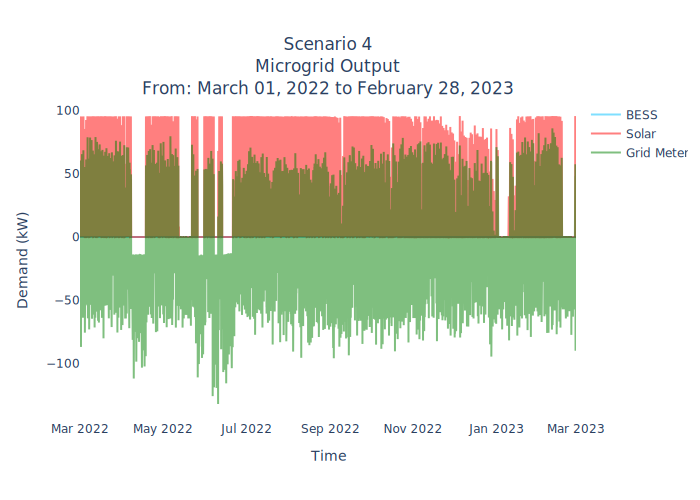
\includegraphics[width=1\linewidth]{Fig/3_Mg_Output_Mar_01_2022_to_Feb_28_2023}
%				\caption{}
%				\label{fig:3mgoutputmar012022tofeb282023}
%			\end{figure}
    		

%\section{Results}
	The microgrid is modified in open Modelica for layout and scenarios. The scenarios are described in Table \ref{tab:scenarios}. Scenarios 1 and 2 are modified in open Modelica directly by shutting down both the solar system and the BESS in scenario 1 and shutting off the BESS in scenario 2. Scenarios 3 -6 by modifying the Python control algorithm open Modelica calls for the BESS. Scenario 3 represents the microgrid's current flat rate pricing structure, while scenarios 4-6 represent different optimizations if our microgrid were under different TOU rates. Each scenario is run independently of one another, and the power outputs of the different components in the simulation are shown in Figure \ref{fig:scenariosubplot}.
%	 \ref{fig:3scenario1mgoutputjun012022tojun302022}, \ref{fig:3scenario2mgoutputjun012022tojun302022}, \ref{fig:3scenario3mgoutputjun012022tojun302022}, \ref{fig:3scenario4mgoutputjun012022tojun302022}, \ref{fig:3scenario5mgoutputjun012022tojun302022}, \ref{fig:3scenario6mgoutputjun012022tojun302022}. 
	 Each scenario's power pulled from the grid is juxtaposed in Figure \ref{fig:netloadscenariocomparisonsummer}, and the daily CO\textsubscript{2} emissions average from each scenario is shown in Figure \ref{fig:emissionsscenariocomparison}. The emissions and electric price amount of each scenario is shown in \ref{tab:emissions}. The CO\textsubscript{2} emissions savings has scenario 1 as a reference since there is no locally-produced renewable energy in this scenario. 
	     	\begin{table}[H]
	 	\caption{Simulated Scenarios of the UCR Microgrid using Different Layouts and Electric Pricing Structures}
	 	\tiny
	 	\begin{tabularx}{\linewidth}{X | l}
\toprule
 Scenario &  \\
\midrule
		1  & No EV Charging with no BESS \\
        2 & Level 2 Charging with no BESS  \\
        3 & Level 3 Charging with no BESS  \\
        4 & Level 2 and Level 3 Charging with no BESS \\
        5 & No EV Charging with BESS \\
        6 & Level 2 Charging with BESS  \\
        7 & Level 3 Charging with BESS \\
        8 & Level 2 and Level 3 Charging with no BESS \\
\bottomrule
\end{tabularx}

	 	\normalsize
	 	\label{tab:scenarios}
	 \end{table}
	 
	 \begin{figure*}
	 	\centering
	 	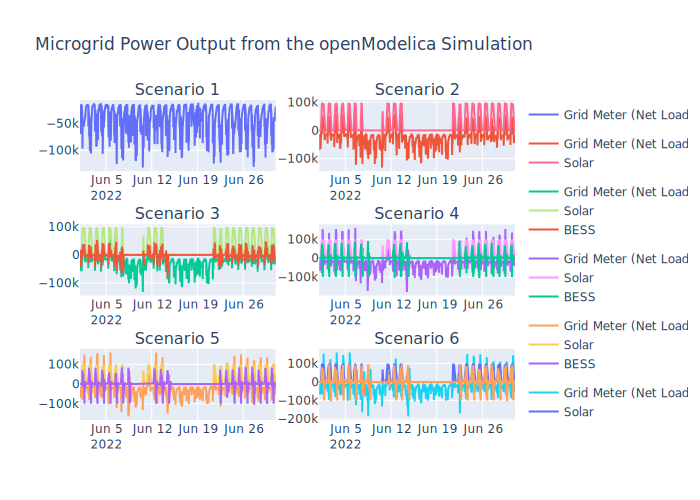
\includegraphics[width=0.9\linewidth]{Fig/scenario_subplot}
	 	\caption{openModelica Power Simulations}
	 	\label{fig:scenariosubplot}
	 \end{figure*}
	
	\begin{table}[H]
		\caption{Microgrid Utility Prices and CO\textsubscript{2} Emissions Output under Different Pricing Scenarios and Pricing Structures}
		\tiny
		\centering
		\resizebox{\columnwidth}{!}{%
		\begin{tabular}{rrrr}
\toprule
 Scenario &  Demand Charges &  Energy Charges &  Emissions \\
\midrule
        1 &            6171 &               0 &         21 \\
        2 &            7963 &            2147 &         25 \\
        3 &           12816 &            2749 &         26 \\
        4 &           14438 &            7274 &         30 \\
        5 &            4992 &               0 &         19 \\
        6 &            6755 &            2925 &         22 \\
        7 &           12053 &            4149 &         23 \\
        8 &           13109 &            8822 &         26 \\
\bottomrule
\end{tabular}

	}
		\normalsize
		\label{tab:emissions}
	\end{table}
	
%     \begin{itemize}
%        \item Pricing table under 4 methods 
%        \item Emissions table under 4 different methods 
%        \item Discuss ideal scenarios under different methods
%        \item Discuss future control methods
%    \end{itemize}   
    
	\begin{figure}[H]
		\centering
		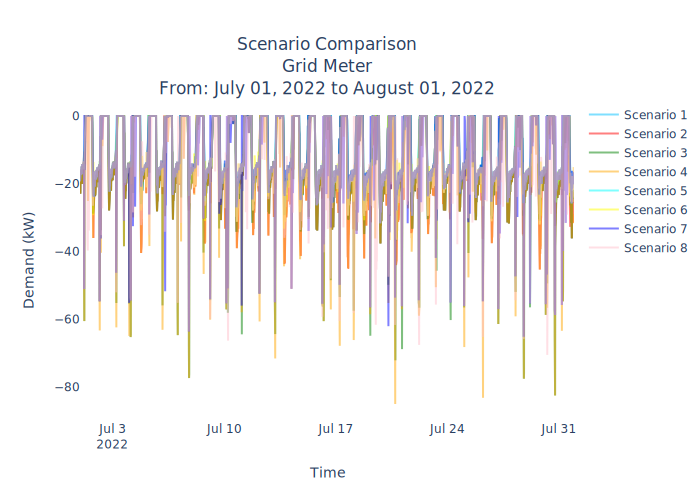
\includegraphics[width=1\linewidth]{Fig/net_load_scenario_comparison_summer}
		\caption{Summer Net Load Scenario Comparison}
		\label{fig:netloadscenariocomparisonsummer}
	\end{figure}
%	\begin{figure}[H]
%		\centering
%		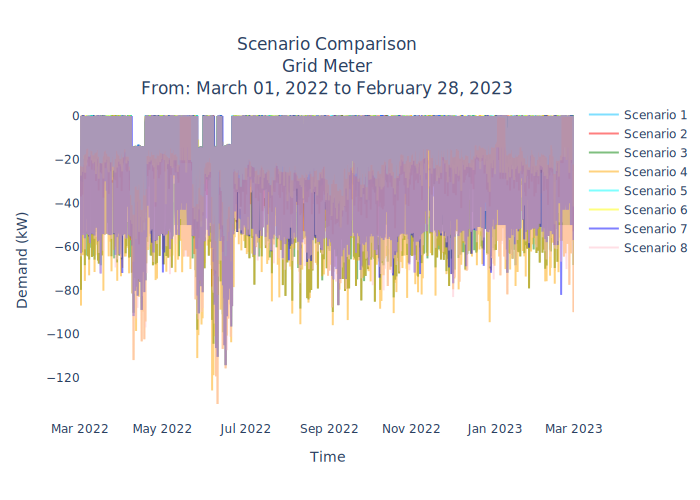
\includegraphics[width=1\linewidth]{Fig/net_load_scenario_comparison}
%		\caption{}
%		\label{fig:netloadscenariocomparison}
%	\end{figure}
	\begin{figure}[H]
		\centering
		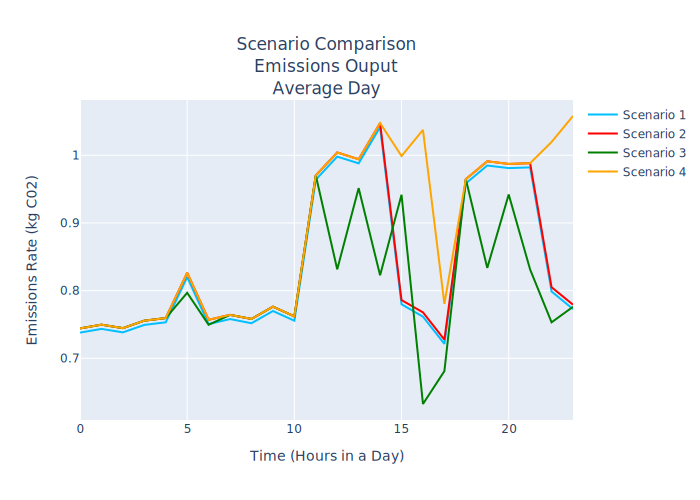
\includegraphics[width=1\linewidth]{Fig/emissions_scenario_comparison}
		\caption{Microgrid  CO\textsubscript{2} Emissions Outputs Averages During Times of Day}
		\label{fig:emissionsscenariocomparison}
	\end{figure}
	\section{Conclusion}
	 The lowest pricing structure for the microgrid customer is SCE's TOU pricing structure, while the lowest emitting setup is standard TOU peak shaving with RPU's flat rate demand cost pricing structure. While adding reliability to any microgrid, a BESS does not always guarantee reduced CO\textsubscript{2} emissions. The opposite is even possible, depending on the pricing structure of the utility. As seen in this paper, all the utility companies have Off-Peak hours during the nighttime, and any price-optimized control algorithm would prioritize charging during that period, so higher net-load peaks occur with a TOU-controlled BESS microgrid. A higher peak during off-peak hours is economically favorable and lower overall demand cost. While current TOU pricing is a great method to mitigate the stress on the grid during on-peak hours, there is major CO\textsubscript{2} production to pricing structure when it comes to microgrids. A balance needs to be met between grid resiliency, lower CO\textsubscript{2} emissions, and profitability. As BESS become more ubiquotus there will a need to make TOU rates with loads that incorporate BESS, as we do right with solar rates. Cheap nighttime off-peak hours incentivize nighttime charging for BESS when the grid in California is most reliant on natural gas for power. A stronger emphasis is also needed on clean nighttime energy, such as wind, geothermal, hydroelectric, and nuclear power, to be further integrated into California's electric grid.
	\section{Future Works}
	Future papers will investigate different microgrid setups and optimizations for a more in-depth analysis.  The effects NEM 3.0 will have on pricing and CO\textsubscript{2} emissions compared to NEM 2.0 is of great interest. Also control algorithms and electric utility TOU rates that can optimize pricing and CO\textsubscript{2} emissions will also be assessed. 
%		\nocite{*}
		\bibliographystyle{IEEEtran}
		\bibliography{cite}
		
\end{document}
